\chapter{Antecedentes}
\label{chap:antecedentes}

En este capítulo se hará un breve estudio del desarrollo de los sistemas empotrados, al estado actual de los mismos, el grado de penetración y uso en el mundo real, los diferentes periféricos que tiene integrado el sistema empotrado sobre el que se va a realizar este \acs{TFG} y el estado actual de los sistemas operativos para sistemas empotrados que existen hoy en día. También se hablará sobre los diferentes sistemas de archivos que existen hoy día, alternativas e historia.\\

\section{Sistemas empotrados}

Un sistema empotrado, también llamado <<sistema embebido>> debido a una mala traducción del anglicismo <<\textit{embedded system}>>, es un sistema computacional diseñado para realizar una o varias tareas muy específicas, generalmente en tiempo real. Al contrario de lo que ocurre con sistemas computacionales de propósito general, que están diseñados para realizar un amplio rango de tareas diferentes, un sistema empotrado está diseñado para cubrir necesidades muy concretas. En un sistema empotrado la mayoría de los componentes están contenidos dentro de la misma placa de silicio y su diseño difiere sustancialmente respecto a lo que solemos asociar con un computador.\\

Un sistema empotrado no está compuesto solo por hardware ya que necesita un software de control capaz de realizar las tareas para las que se diseña. Generalmente este software de control se desarrolla a la vez que el sistema hardware para poder ajustarse a los requisitos, aunque en los últimos tiempos este paradigma está cambiando al aparecer en el mercado placas que pueden ser reprogramadas y ser orientadas a multitud de diferentes tareas. \\ 

Los sistemas de este tipo, al estar pensados para hacer tareas concretas, suelen tener unas restricciones de memoria y capacidad de cómputo ajustadas a las tareas que se pretende que realicen para así controlar y reducir los costes de fabricación. \\

Normalmente estos sistemas son reactivos y funcionan en tiempo real, entendiendo por reactivo un sistema que interactúa con el entorno cuando se produce un evento predeterminado y funcionar en tiempo real que el comienzo de la acción a realizar sucede en un período de tiempo acotado desde que sucedió el evento que la produjo \cite{EmbeddedOS}.\\

Los componentes fundamentales de un sistema empotrado clásico son una memoria para almacenar el programa de control, un procesador para poder ejecutarlo y buses de comunicación entre los componentes sobre los que se pueden conectar otros componentes externos como pueden ser sensores, actuadores u otros sistemas empotrados \cite{EmbeddedOS}.\\



\section{Desarrollo de sistemas empotrados}
\label{sec:3.2}
El desarrollo de los Sistemas Empotrados difiere sustancialmente del desarrollo del software convencional, no sólo por las restricciones de memoria y capacidad de cómputo de estos sistemas sino por la estructura física de este tipo de componentes que puede hacer inviable la utilización de componentes que funcionarían a la perfección en sistemas de propósito general.\\

El desarrollo de un sistema empotrado empieza por la definición de las tareas que debe realizar seguido de un estudio pormenorizado de las necesidades computacionales y de memoria que se necesitan, así como los periféricos, sensores y actuadores que se tienen que controlar y monitorizar para realizar las tareas propuestas.\\

El proceso de desarrollo de un sistema empotrado se suele realizar \textit{top-down}, comenzando con la especificación del sistema completo y en iteraciones posteriores ir bajando el nivel de abstracción hasta tener el sistema completo bien definido, pasando, en este orden, por la especificación a nivel de sistema, a nivel de computación, a nivel lógico y por último a nivel de circuito.\\

Existen otras metodologías más clásicas como puede ser \textit{bottom-up}, en la que se empieza a desarrollar desde un nivel de abstracción menor hacia uno mayor, o \textit{meet in the middle} donde se combinan las metodologías \textit{top-down} y \textit{bottom-up} intentando suplir las carencias de cada una y sumando sus ventajas.\\

Si a estas metodologías le añadimos un componente de pruebas tenemos la que más se utiliza en el desarrollo de este tipo de sistemas y a la que se le suele llamar \acf{SER} \cite{embDes}. \\

El flujo de trabajo de la metodología \acs{SER} se especifica a continuación:
\begin{itemize}
\item Especificación ejecutable a nivel de sistema, representando el comportamiento del mismo.
\item Incluir varios modelos con diferentes detalles que corresponden a diferentes decisiones de diseño (propiedades del sistema tales como velocidad, consumo de potencia, etc).
\item Síntesis de las diferentes opciones para explorar el espacio de diseño.
\item Refinamiento del modelo de acuerdo a las decisiones tomadas.\\
\end{itemize}

En la figura \ref{fig:DisSistEmp} podemos ver las tareas que se necesitan completar para realizar el diseño de un sistema empotrado completo. En el caso del sistema empotrado objetivo de este \acs{TFG} la rama de desarrollo del hardware no es necesario realizarla ya que se utiliza una placa ya existente. \\

\begin{figure}[!h]
\begin{center}
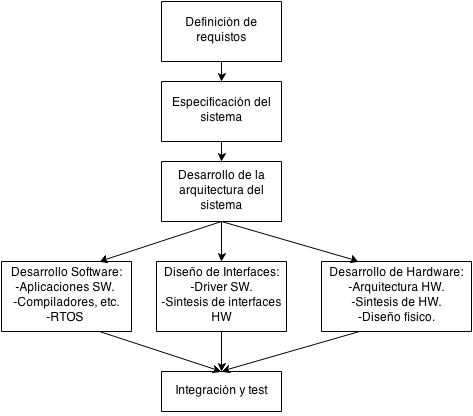
\includegraphics[width=0.7\textwidth]{figs/DisSistEmp.png}
\caption{Diagrama de flujo del desarrollo de un sistema empotrado}
\label{fig:DisSistEmp}
\end{center}
\end{figure}

Otra metodología de desarrollo, y más adecuada para la realización de este \acs{TFG} es el llamado <<Desarrollo de Sistemas Basado en Placa>>, donde el desarrollo del hardware es totalmente independiente del desarrollo del software y pueden estar realizados por diferentes equipos de trabajo \cite{embDes}. Esta metodología tiene la ventaja que la placa hardware obtenida puede ser utilizada para diversas funcionalidades, y el inconveniente principal es que se pueden encontrar restricciones que obliguen a cambiar el diseño original del sistema. Utilizando esta metodología, el equipo de desarrollo del componente software puede utilizar cualquier metodología clásica de desarrollo de software, aunque no podrá aplicarla completamente debido a las características propias del desarrollo de este tipo de sistemas. En el Capítulo \ref{chap:metodo} se detalla la metodología utilizada para el desarrollo de este \acs{TFG}, los inconvenientes que han surgido y cómo se han solucionado.\\

\section{Historia e importancia de los sistemas empotrados}

Los sistemas empotrados conviven con nosotros desde los ‘60 cuando el \acf{MIT} desarrolló el primer sistema empotrado para controlar el sistema de guía del proyecto Apolo \cite{website:mitApolo}. Desde entonces han servido para automatizar los más diversos procesos y ofreciendo herramientas de las que no se disponía hasta entonces. Los sistemas empotrados se encuentran en todos los dispositivos electrónicos que nos rodean, desde juguetes, teléfonos móviles y televisiones, hasta los sistemas de control de una fábrica, de un vehículo de transporte (trenes, aviones, coches, barcos, ..) o de los semáforos que controlan el tráfico.\\

Los sistemas empotrados de hoy día pueden realizar muchas más tareas que los primeros que se desarrollaron ya que la evolución de la tecnología ha permitido no solo el abaratamiento de los componentes sino que también ha permitido aumentar enormemente su rendimiento llegando al punto que algunos sistemas empotrados, como los llamados \textit{smartphones}, igualan o superan a sistemas de propósito general realizando tareas similares \cite{website:AndroidLikeSuperComputer}.\\

Como hemos visto anteriormente, este tipo de sistemas están diseñados para realizar solo unas cuantas tareas específicas cada uno pero se pueden utilizar en multitud de áreas y campos. \\

La utilización de los sistemas empotrados en productos electrónicos suele solventar problemas de complejidad y de tamaño del producto. Por ejemplo un automóvil actual contiene docenas de sistemas empotrados para controlar diferentes aspectos del mismo, como el aire acondicionado, la inyección de combustible o la presión de las ruedas. Si los automóviles no tuvieran estos sistemas empotrados la lógica de control sería mucho más compleja y propensa a fallos. Otra alternativa sería tener un sistema computacional de propósito general, pero estaría sobredimensionado y aumentaría notablemente los costes de producción \cite{EmbeddedOS}.\\


\section{Componentes de un sistema empotrado}

Todos los sistemas empotrados tienen una serie de componentes comunes entre sí:

\begin{itemize}
\item Software de control.
\item Microprocesador para poder ejecutar el software.
\item Memoria volátil (RAM) para la memoria del programa durante la ejecución.
\item Memoria no volátil (generalmente FLASH) para almacenar datos persistentes y/o el binario ejecutable del software de control.
\item Subsistema de entrada/salida, utilizado para comunicarse con componentes externos como actuadores y sensores.
\begin{itemize}
\item Sensores: estos componentes únicamente miden magnitudes físicas. Ejemplos de este tipo pueden ser un GPS o un termómetro.
\item Actuadores: estos componentes son capaces de relacionarse con el mundo físico y realizar cambios sobre él. En este tipo de componentes se encuentran todos los componentes que interactúan con el usuario, como pueden ser un dispositivo Bluetooth o un \textit{display}, o con el medio físico, como puede ser un motor, una alarma o una luz.
\item Existen otro tipo de componentes que se pueden conectar a un sistema empotrado pero que no se pueden catalogar ni como actuadores ni como sensores. Entre este tipo de componentes podemos encontrar, por ejemplo, las memorias externas u otros sistemas empotrados.\\
\end{itemize}
\end{itemize}

En la Figura \ref{fig:CapasSistemaEmpotrado} podemos ver cómo se relacionan entre sí los diferentes componentes de un sistema empotrado.\\

\begin{figure}[!h]
\begin{center}
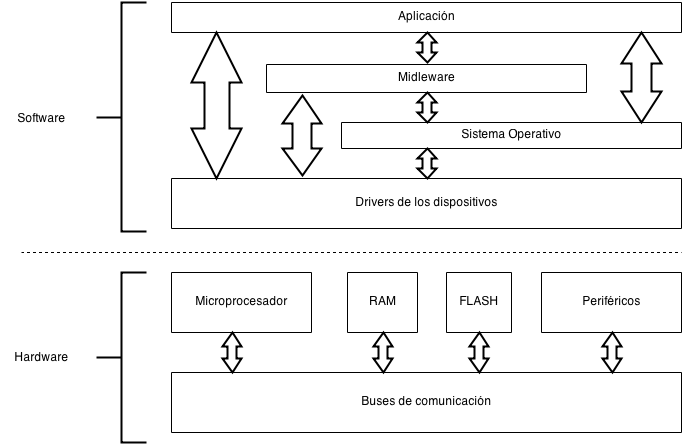
\includegraphics[width=0.7\textwidth]{figs/CapasSistemaEmpotrado.png}
\caption{Diagrama de interacción entre componentes de un Sistema Empotrado}
\label{fig:CapasSistemaEmpotrado}
\end{center}
\end{figure}

\section{Sistemas Operativos para Sistemas Empotrados}

Un Sistema Operativo es un programa entre cuyas responsabilidades se encuentran ser una capa de abstracción del hardware, gestionar los permisos y tiempos de acceso a los dispositivos, gestionar la ejecución de tareas que funcionan sobre él, la gestión de la memoria que puede utilizar cada tarea o el soporte de varios usuarios, entre otras muchas.\\

Un Sistema Operativo para un sistema empotrado debe ser mucho más liviano que para un sistema de propósito general debido fundamentalmente a las restricciones de cómputo mencionadas. Un Sistema Operativo de este tipo solo puede hacer las funciones más básicas como puede ser la gestión de la ejecución de las tareas, concretamente del cambio de contexto de ejecución de una tarea a otra.\\

Muchos sistemas empotrados que no tienen fuertes restricciones de memoria y cómputo utilizan sistemas operativos completos como pueden ser Linux~\cite{website:linux}, Android~\cite{website:Android} o iOS~\cite{website:iOS}.\\

En caso que el sistema empotrado objetivo ejecute únicamente una tarea entonces el Sistema Operativo puede no existir, disminuyendo así los requisitos computacionales necesarios para su correcto funcionamiento. Si el sistema tiene que realizar muy pocas tareas y se considera que no es necesario un Sistema Operativo, entonces necesitamos diseñar y programar un sistema que cambie el contexto de ejecución correctamente, como puede ser un sistema de \textit{polling} que cambie de contexto de manera automática y periódica con un tiempo preestablecido.\\

Si el sistema empotrado objetivo ejecuta un número considerable de tareas o necesita ejecutarlas en tiempo real entonces necesitaremos un sistema operativo acorde las necesidades impuestas para facilitar la tarea de desarrollo. Uno de los sistemas operativos para sistemas empotrados más utilizados es FreeRTOS \cite{website:FreeRTOS}, un sistema operativo en tiempo real liberado con una licencia \acf{GPL}, pero hay muchos otros como pueden ser TinyOs \cite{website:tinyOS}, eCos \cite{website:ecOS} o chibiOS \cite{website:chibios}.\\

En general, los Sistemas Operativos para sistemas empotrados tienen una estructura y funcionamiento común. El desarrollador del sistema debe separar las funcionalidades requeridas en diferentes tareas y el sistema se encargará de gestionar el uso de los recursos requeridos por cada una, dependiendo de sus prioridades.\\

Para gestionar la comunicación entre las diferentes tareas de un Sistema Operativo suelen ofrecer los mecanismos típicos de sincronización y comunicación, como son los semáforos, y las colas de mensajes.\\


\section{Sistemas de Archivos}
Un sistema de archivos es una abstracción del almacenamiento en memoria que permite manejarla con mucha más facilidad. Un sistema de archivos permite gestionar, organizar y buscar archivos, así como realizar operaciones de lectura y escritura sobre los mismos.\\

Uno de los primeros sistemas de archivos que apareció en el mercado fue FAT, introducido en 1977 por Microsoft para su sistema DOS. Este sistema de archivos se sigue utilizando ampliamente en la actualidad, sobretodo en dispositivos de almacenamiento de memoria externos como las memorias FLASH USB. FAT, como la totalidad de sistemas de archivos posteriores, divide la memoria disponible en sectores de tamaño fijo y configurable, siendo ésta la unidad mínima de trabajo tanto para leer, escribir o borrar. La forma de almacenar la información sobre los archivos que tiene FAT es guardándolo en una tabla en la que cada fila representa, en orden, los sectores en los que se divide la memoria y cada entrada especifica si está libre u ocupado y de estarlo el fichero al que se refiere y dónde encontrar el siguiente sector ocupado que corresponde al mismo archivo (Figura \ref{fig:fatTable}).\\

Posteriormente aparecieron nuevos sistemas de archivos que permitían operaciones sobre archivos más rápidas y más complejas, nombres más largos y con diferente codificación, inclusión de metadatos, y soporte para cantidades de memoria cada vez mayores. También evolucionaron sistemas de archivos más antiguos como FAT que dio lugar a FAT16 y posteriormente a FAT32 \cite{website:fat}.\\

\begin{figure}[!h]
\begin{center}
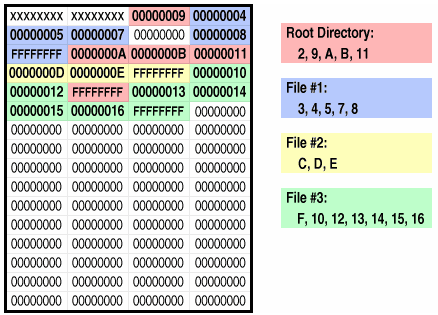
\includegraphics[width=0.7\textwidth]{figs/fatTable.png}
\caption{Tabla de asignación de archivos del Sistema de Archivos FAT}
\label{fig:fatTable}
\end{center}
\end{figure}

Actualmente Microsoft utiliza en sus productos el sistema de archivos NTFS \cite{website:ntfs}, privativo y sin soporte oficial para otros sistemas operativos pero del que, gracias a la ingeniería inversa, se ha conseguido entender su funcionamiento y ofrecer un soporte no oficial.\\

Para los sistemas Linux se utilizan muy diversos sistemas de archivos dependiendo del propósito del computador en cuestión. Uno de los más usados es ext4 \cite{website:ext4}, introducido en 2008 y evolución del sistema ext, el primer sistema de archivos soportado por Linux e introducido en 1992, y que soporta particiones de hasta un petabyte de tamaño y archivos de hasta 16 TBytes. El funcionamiento de este sistema de archivos es mediante \textit{extents}, una agrupación de sectores de hasta 120 MB, pudiéndose almacenar hasta 4 en el descriptor de archivo pero, en el caso de que fueran necesarios más, uno de ellos puede referirse a otra dirección de memoria donde se almacenarían otros nuevos 4 \textit{extents}, funcionando como si de un árbol se tratara (Figura \ref{fig:HTree}).\\

\begin{figure}[!h]
\begin{center}
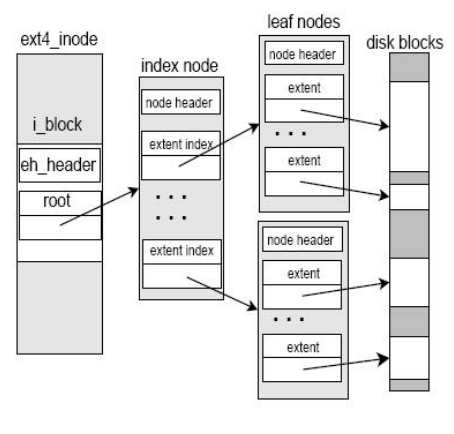
\includegraphics[width=0.5\textwidth]{figs/HTree.png}
\caption{Representación gráfica del funcionamiento de HTree}
\label{fig:HTree}
\end{center}
\end{figure}

Para un sistema empotrado, donde la capacidad de cómputo y la memoria disponible son muy reducidas, es posible que no convenga utilizar sistemas de archivos tan avanzados como ext4 y funcionen mejor sistemas como FAT, pero todo dependerá de las características y requisitos del sistema a desarrollar.\\

Hay que tener en cuenta, además, que la arquitectura de la memoria embebida en el sistema puede hacer inviable la utilización de cualquiera de los estándares definidos para la implementación de un Sistema de Archivos.\\

Otro aspecto a tener en cuenta para el desarrollo de un Sistema de Archivos es la arquitectura física de la memoria y su tecnología de fabricación. Los sistemas de archivos, aunque su funcionamiento básico sea el mismo, deben diferenciar el tipo de memoria sobre el que trabajan para proporcionar un mayor rendimiento y fiabilidad.\\
 
Actualmente el desarrollo de los nuevos Sistemas de Archivos viene impuesto por el avance, tanto en costes como en rendimiento, de las memorias FLASH utilizadas en discos SSD, de varios TBytes. Esta tecnología, además presenta dos variantes que se deben tener en cuenta a la hora de implementar los drivers de acceso, y son la fabricación mediante NAND o mediante NOR.\\

Los sistemas empotrados, generalmente, llevan memoria FLASH embebida, por lo que es relevante para la realización de este \acs{TFG} hacer un repaso sobre los sistemas de archivos desarrollados para esta tecnología, aunque suelen ser modificaciones sobre sistemas de archivos de propósito general.\\

Para memorias FLASH en general tenemos como ejemplo de sistema de archivos específico JFFS2 \cite{website:JFFS2}, que soporta el formato de metadatos de POSIX y comprime los datos durante las escrituras.\\

Para memorias FLASH fabricadas con tecnología NAND tenemos YAFFS2 \cite{website:YAFFS2}, una modificación de JFFS2 diseñadas específicamente para este tipo de memorias. \\

También hay alternativas de sistemas de archivos de solo lectura que pueden ser útiles en determinados entornos, como pueden ser ROMFS \cite{website:romfs} o SQUASHFS \cite{website:squashfs}.\\



\section{Dispositivos GPS}

El Sistema de Posicionamiento Global (GPS) es un sistema propietario y privativo del gobierno de Estados Unidos, construido pensando en el uso militar, que es capaz de determinar la posición de un dispositivo compatible proporcionándole la información sobre la latitud, longitud y altitud a la que se encuentra \cite{website:GPS}.\\


El Sistema GPS funciona gracias a 24 satélites en órbita sobre el planeta Tierra, con trayectorias sincronizadas, que envían constantemente señales hacia la Tierra. El método para determinar la posición exacta sobre la Tierra es mediante triangulación inversa de varias de estas señales. Esto exige que el sistema se encuentre al alcance de la señal de al menos tres de estos satélites, lo que implica que la mayoría de los dispositivos no funcionen de forma correcta en interiores y necesiten ayuda de una antena exterior. \cite{website:GPS}.\\

La Unión Soviética empezó a construir un sistema similar, llamado GLONASS, que no consiguió terminar hasta 2007. También pensado para uso exclusivamente militar pero liberado posteriormente para uso civil.\\

La Unión Europea está desarrollando otro sistema similar, llamado Galileo. Este sí será el primer sistema de geoposicionamiento motivado desde el principio para uso civil. Este sistema, además, implementa una mejora de precisión sobre los sistemas GPS y GLONASS cuando se consulta la posición en los polos.\\

China está desarrollando también una alternativa a los sistemas existentes, llamado BEIDOU. Este sistema difiere bastante de los anteriores ya que sus satélites se encuentran en zona geoestacionaria (los satélites del resto de sistemas se encuentran más bajos) y para el cálculo de la posición sobre la Tierra hace uno de dos de esos satélites y de una estación en tierra. La posición geoestacionaria de sus satélites garantiza un correcto funcionamiento con muy pocos satélites, pero limita su cobertura sobre la tierra a la visible por los satélites, Actualmente este sistema solo tiene una cobertura sobre toda China y algunos países circundantes.\\

Actualmente podemos encontrar dispositivos GPS en casi cualquier dispositivo electrónico, desde el más sencillo smartphone hasta vehículos como coches, barcos, trenes, aviones, etc., y en dispositivos específicos hechos para la lectura de datos GPS y la ayuda a la realización de rutas como pueden ser los dispositivos comercializados por la empresa TOMTOM.\\

Recientemente, además, están apareciendo dispositivos compatibles con varios de los sistemas de geoposicionamiento global existentes.\\

El estándar de transmisión de datos GPS es el NMEA 0183, como se verá más concretamente en el apartado \ref{sec:dispGPS}.\\



